% !TeX root = ../main.tex

\chapter{多智能体协同、Skill 封装与工具调用设计}
\label{sec:multi-agent}

\definecolor{chthreeaccent}{HTML}{E9E9F5}
\tikzset{
  cthreebox/.style={draw=black!70, rounded corners=2pt, fill=white, align=center, minimum height=0.92cm, text width=2.35cm, font=\small},
  cthreemain/.style={draw=black!78, rounded corners=2pt, fill=chthreeaccent, align=center, minimum height=1.02cm, text width=2.55cm, font=\small\bfseries},
  cthreedata/.style={draw=black!58, rounded corners=2pt, fill=black!5, align=center, minimum height=0.88cm, text width=2.5cm, font=\small},
  cthreewarn/.style={draw=black!70, rounded corners=2pt, fill=black!8, align=center, minimum height=0.88cm, text width=2.55cm, font=\small},
  cthreearrow/.style={->, >=stealth, thick, draw=black!78},
  agentinput/.style={draw=black!72, line width=.65pt, rounded corners=2pt, fill=white, align=center, minimum height=1.02cm, text width=2.25cm, font=\scriptsize},
  agentcore/.style={draw=black!78, line width=.8pt, rounded corners=2pt, fill=chthreeaccent, align=center, minimum height=1.08cm, text width=2.35cm, font=\scriptsize\bfseries},
  agentprocess/.style={draw=black!68, line width=.65pt, rounded corners=2pt, fill=black!3, align=center, minimum height=1.02cm, text width=2.2cm, font=\scriptsize},
  agentoutput/.style={draw=black!72, line width=.65pt, rounded corners=2pt, fill=white, align=center, minimum height=1.02cm, text width=2.3cm, font=\scriptsize},
  agentmemory/.style={draw=black!55, line width=.55pt, rounded corners=2pt, fill=black!5, align=center, minimum height=.72cm, text width=4.0cm, font=\scriptsize},
  agentarrow/.style={->, >=stealth, line width=.7pt, draw=black!78},
  agentfeedback/.style={->, >=stealth, line width=.65pt, dashed, draw=black!58}
}

\section{学习资源 Agent 设计与协作}

OralSage 围绕口腔医学主题学习展开路径规划、材料组织、连续讲解、即时答疑、理解检验和章节推进等相互衔接的教学活动。学习资源 Agent 群围绕同一学习会话协同工作，课程单元、讲义章节、知识图谱关系、学习进展和答题表现持续贯穿各个环节。学习者既能围绕当前需求启动某项专业能力，也能从一个主题进入具有完整结构的连续课程，系统会在不同学习时刻调动最契合的 Agent 参与教学。

这种设计让学习资源从静态内容扩展为动态生长的教学环境。课程规划提供知识理解的主线，讲义与多模态材料丰富学习媒介，讲解与答疑持续深化理解，测评与后续章节共同推动学习进展。对学习者而言，每一轮学习活动都能够回到当前主题、当前章节和当前学习状态，既保持课程结构的连续性，也保留按需探索的灵活性。

\begin{figure}[H]
  \centering
  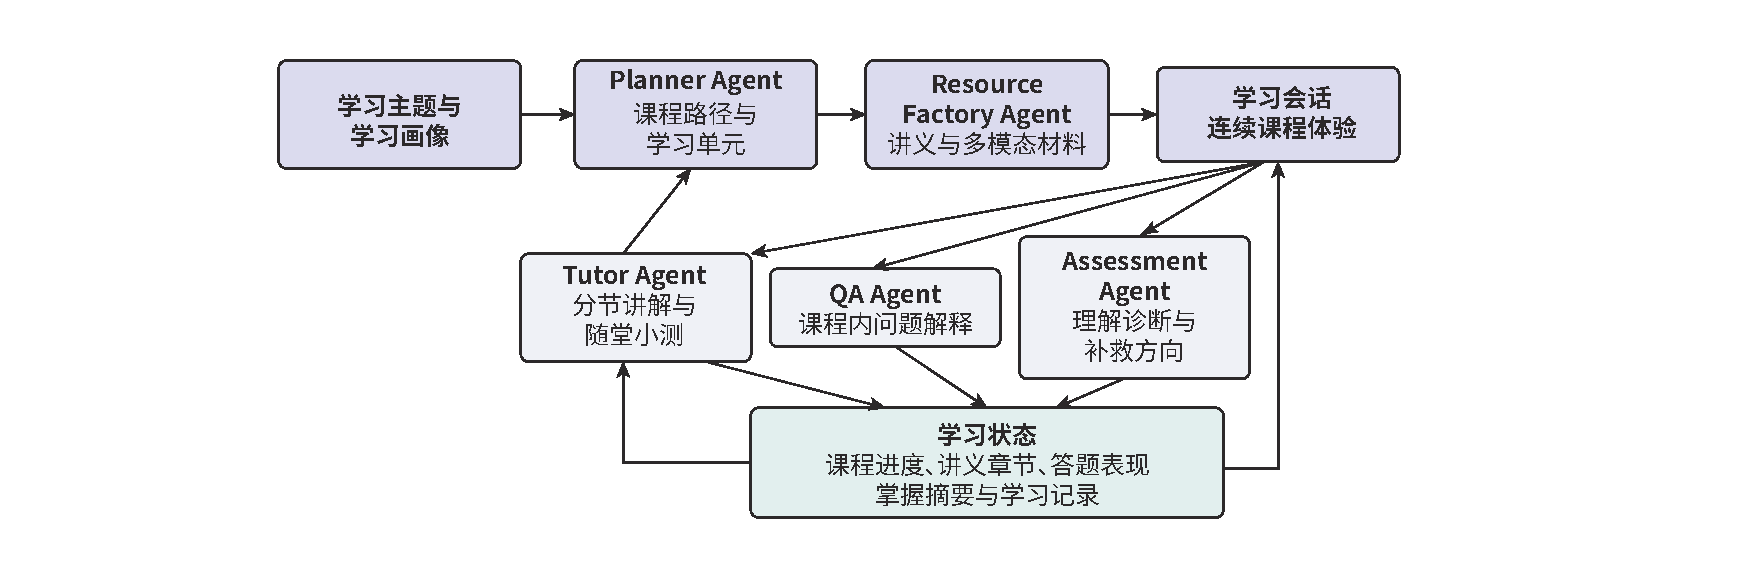
\includegraphics[width=0.96\linewidth]{Collaboration-between-learning-resources-and-agents.pdf}
  \caption{学习资源 Agent 群的协同关系}
  \label{fig:agent-overall-architecture}
\end{figure}

\subsection{Planner Agent}

主题进入课程后，Planner Agent 会综合学习主题、学习者画像、知识图谱节点、概念关系、资料片段和关联题目，编织由多个学习单元组成的课程路径。每个单元都围绕明确的理解目标展开，编排理由、知识范围和资料范围也会写入单元设计。口腔医学中病因机制、临床表现、诊断思路与治疗原则之间存在天然依赖，课程顺序能够沿着知识结构逐步展开，帮助学习者从概念建立走向重点理解。

Planner Agent 为整个学习资源体系确立共同教学语境，使 Resource Factory 能够围绕当前章节准备材料，Tutor 能够承接前后章节进行讲解，QA 能够理解问题所处的课程位置，Assessment 能够把作答表现映射到相关知识内容。对学习者而言，Planner Agent 的核心价值不只是排列课程单元，而是把分散的知识、资料和题目组织成一条可以执行的学习路径。学习者无需反复判断“先学什么、后学什么”，即可沿着清晰的主线逐步完成主题学习。

\begin{figure}[H]
  \centering
  \resizebox{\linewidth}{!}{%
  \begin{tikzpicture}[node distance=.5cm and .48cm]
    \node[font=\small\bfseries] at (6.85,1.25) {Planner Agent 工作流};
    \node[agentinput] (pinput) at (0,0) {主题学习请求\\学习画像与课程进展};
    \node[agentcore, right=of pinput] (pcontext) {主题语境聚合\\知识关系、资料与题目};
    \node[agentprocess, right=of pcontext] (pstructure) {知识结构编排\\前后概念依赖与重点};
    \node[agentcore, right=of pstructure] (punit) {学习单元设计\\目标、顺序与学习范围};
    \node[agentoutput, right=of punit] (ppath) {课程路径\\可进入的首个学习单元};
    \node[agentmemory, below=1.0cm of pstructure] (pmemory) {学习状态回流：章节进展、答题表现、掌握摘要与互动历史};
    \draw[agentarrow] (pinput) -- (pcontext);
    \draw[agentarrow] (pcontext) -- (pstructure);
    \draw[agentarrow] (pstructure) -- (punit);
    \draw[agentarrow] (punit) -- (ppath);
    \draw[agentfeedback] (ppath.south) |- (pmemory.east);
    \draw[agentfeedback] (pmemory.west) -| (pcontext.south);
  \end{tikzpicture}}
  \caption{Planner Agent 的课程路径规划工作流}
  \label{fig:planner-workflow}
\end{figure}

\subsection{Resource Factory Agent}

课程路径确定后，Resource Factory Agent 围绕学习单元组织讲义、课件、讲稿、语音、思维导图和练习材料。讲义生成遵循“资料规划、内容写作”的两阶段教学策略。前一阶段聚焦本节核心知识、资料组合和表达重点，后一阶段依据已经准备好的资料组织具有教学层次的讲义内容。课程目标、知识关系和重点概念持续贯穿材料生成过程，学习者能够在内容中感受到清晰的专业表达和稳定的章节主题。

同一学习单元还会延展出讲义、课件、文字讲解、语音讲解和思维导图等多种媒介形态。这些材料分别承担理论梳理、重点呈现、听觉讲解和复习辅助等作用，共同帮助学习者建立知识框架、理解重点内容，并完成后续练习与复习。学习者可以在阅读、浏览、听讲和练习之间自然切换，而不必重新寻找与当前主题对应的学习材料。首节优先的准备节奏进一步缩短主题学习的启动时间，随着课程推进，课程材料持续丰富，使课程体验兼具完整性和流畅性。

\begin{figure}[H]
  \centering
  \resizebox{\linewidth}{!}{%
  \begin{tikzpicture}[node distance=.5cm and .48cm]
    \node[font=\small\bfseries] at (6.85,1.25) {Resource Factory Agent 工作流};
    \node[agentinput] (rinput) at (0,0) {学习单元\\目标、范围与知识关系};
    \node[agentcore, right=of rinput] (rplan) {资料规划\\重点概念与材料组合};
    \node[agentprocess, right=of rplan] (rwrite) {教学内容组织\\层次、节奏与表达重点};
    \node[agentcore, right=of rwrite] (rmedia) {多媒介延展\\讲义、课件、讲稿、语音};
    \node[agentoutput, right=of rmedia] (rresult) {学习资源包\\围绕单元一致呈现};
    \node[agentmemory, below=1.0cm of rwrite] (rstate) {课程语境贯穿：当前章节、学习主题、概念脉络与后续活动};
    \draw[agentarrow] (rinput) -- (rplan);
    \draw[agentarrow] (rplan) -- (rwrite);
    \draw[agentarrow] (rwrite) -- (rmedia);
    \draw[agentarrow] (rmedia) -- (rresult);
    \draw[agentfeedback] (rresult.south) |- (rstate.east);
    \draw[agentfeedback] (rstate.west) -| (rplan.south);
  \end{tikzpicture}}
  \caption{Resource Factory Agent 的多媒介资源生成工作流}
  \label{fig:resource-factory-workflow}
\end{figure}

\subsection{Tutor Agent}

Tutor Agent 通过承接讲义内容、前后章节关系、学习位置、相关知识节点和掌握摘要，以更贴近教学语言的方式展开分节讲解，使得病因机制、临床表现、诊断思路和治疗原则之间的关联能够在连续表达中逐步展开，学习者既能理解当前概念，也能把握其与前后知识内容之间的联系。章节过渡、重点提示和即时小测共同让每一次讲解保持清晰的学习焦点。

学习者可以直接发起当前章节讲解，或根据自己的理解情况请求调整表达方式；Tutor 也会随着总控调度伴随课程进展持续出现。由于讲解始终承接当前章节、学习位置和已有掌握情况，学习者不需要每次重新说明背景，就可以继续上一次学习过程。每一轮讲解既承担知识解释，也承担学习节奏提示，使学习者能够持续感知已经理解的内容、正在学习的位置和下一步方向，形成接近一对一辅导的连续体验。

\begin{figure}[H]
  \centering
  \resizebox{\linewidth}{!}{%
  \begin{tikzpicture}[node distance=.5cm and .48cm]
    \node[font=\small\bfseries] at (6.85,1.25) {Tutor Agent 工作流};
    \node[agentinput] (tinput) at (0,0) {当前学习单元\\讲义内容与学习位置};
    \node[agentcore, right=of tinput] (tprepare) {教学语境组织\\概念关系与掌握摘要};
    \node[agentprocess, right=of tprepare] (texplain) {分节讲解推进\\机制、表现、思路与原则};
    \node[agentcore, right=of texplain] (tinteract) {互动教学调节\\重点提示、过渡与即时小测};
    \node[agentoutput, right=of tinteract] (tresult) {连续讲解体验\\理解当前位置与下一步方向};
    \node[agentmemory, below=1.0cm of texplain] (tstate) {学习信号回流：讲解进度、互动偏好、理解摘要与章节状态};
    \draw[agentarrow] (tinput) -- (tprepare);
    \draw[agentarrow] (tprepare) -- (texplain);
    \draw[agentarrow] (texplain) -- (tinteract);
    \draw[agentarrow] (tinteract) -- (tresult);
    \draw[agentfeedback] (tresult.south) |- (tstate.east);
    \draw[agentfeedback] (tstate.west) -| (tprepare.south);
  \end{tikzpicture}}
  \caption{Tutor Agent 的连续讲解工作流}
  \label{fig:tutor-workflow}
\end{figure}

\subsection{QA Agent}

用户进行提问之后，系统调用 QA Agent，将当前问题与正在学习的单元、讲义内容、知识图谱关系、相关资料和近期对话联系在一起。围绕病因机制、概念辨析、检查思路或治疗原则等问题，QA 会先判断提问与当前章节之间的联系，再结合课程资料和主题检索展开解释。这样，学习者得到的不是脱离课程上下文的孤立答案，而是能够回到当前知识结构中的针对性说明，在解决眼前困惑的同时继续推进对主题的理解。


\begin{figure}[H]
  \centering
  \resizebox{\linewidth}{!}{%
  \begin{tikzpicture}[node distance=.5cm and .48cm]
    \node[font=\small\bfseries] at (6.85,1.25) {QA Agent 工作流};
    \node[agentinput] (qinput) at (0,0) {课程内追问\\当前单元与近期对话};
    \node[agentcore, right=of qinput] (qidentify) {问题语境辨析\\问题与章节位置关联};
    \node[agentprocess, right=of qidentify] (qretrieve) {主题资料联结\\讲义、知识关系与相关资料};
    \node[agentcore, right=of qretrieve] (qanswer) {深入解释组织\\概念辨析与机制阐释};
    \node[agentoutput, right=of qanswer] (qreturn) {回归课程主线\\带着理解继续学习};
    \node[agentmemory, below=1.0cm of qretrieve] (qstate) {课程语境保持：正在学习的章节、问题脉络与知识范围};
    \draw[agentarrow] (qinput) -- (qidentify);
    \draw[agentarrow] (qidentify) -- (qretrieve);
    \draw[agentarrow] (qretrieve) -- (qanswer);
    \draw[agentarrow] (qanswer) -- (qreturn);
    \draw[agentfeedback] (qreturn.south) |- (qstate.east);
    \draw[agentfeedback] (qstate.west) -| (qidentify.south);
  \end{tikzpicture}}
  \caption{QA Agent 的课程内即时解释工作流}
  \label{fig:qa-workflow}
\end{figure}

\subsection{Assessment Agent}

提交作答后，Assessment Agent 先核对选项与答案，再结合题目考查内容解释关键判断依据。出现偏差时，系统会定位容易混淆的概念，并把相关知识点和复习方向带回当前学习单元；答对时，则以简短提示强化本题的判断线索。练习结果能够转化为下一步学习的具体着力点。

Assessment Agent 能够将学习者的答题表现、相关知识点和知识点巩固方向写进学习状态中，使后续 Tutor 讲解、QA 追问和课程路径调节获得更具针对性的学习信号。对学习者而言，练习结果不再只是一次性的对错反馈，而会进一步转化为“哪些概念已经掌握、哪些地方容易混淆、下一步应该复习什么”的学习提示，成为知识掌握、学习反馈和后续学习之间的重要连接点。

\begin{figure}[H]
  \centering
  \resizebox{\linewidth}{!}{%
  \begin{tikzpicture}[node distance=.5cm and .48cm]
    \node[font=\small\bfseries] at (6.85,1.25) {Assessment Agent 工作流};
    \node[agentinput] (ainput) at (0,0) {练习作答\\当前主题与题目语境};
    \node[agentcore, right=of ainput] (ajudge) {作答理解\\选项识别与正误判断};
    \node[agentprocess, right=of ajudge] (aanalyze) {理解诊断\\误区、知识缺口与关联概念};
    \node[agentcore, right=of aanalyze] (adirect) {学习建议组织\\解析、复习重点与补救方向};
    \node[agentoutput, right=of adirect] (aresult) {学习推进信号\\服务后续讲解与课程调节};
    \node[agentmemory, below=1.0cm of aanalyze] (astate) {掌握状态更新：作答表现、薄弱知识点、复习方向与课程进展};
    \draw[agentarrow] (ainput) -- (ajudge);
    \draw[agentarrow] (ajudge) -- (aanalyze);
    \draw[agentarrow] (aanalyze) -- (adirect);
    \draw[agentarrow] (adirect) -- (aresult);
    \draw[agentfeedback] (aresult.south) |- (astate.east);
    \draw[agentfeedback] (astate.west) -| (ajudge.south);
  \end{tikzpicture}}
  \caption{Assessment Agent 的理解诊断与学习推进工作流}
  \label{fig:assessment-workflow}
\end{figure}

\subsection{叶子 Agent 群设计}

为了更好地协调学习系统的各类能力，OralSage 设计了叶子 Agent 群。这里的“叶子 Agent”是指能够直接完成某一项具体学习服务、也能够被上层课程流程组合调用的基础能力单元。它们把学习资源交付和学习推进拆解为一组可独立调用的专业能力。学习者可以根据当下需求快速获得讲义、课件、演示文稿、讲稿、语音、练习或继续学习体验；进入系统化主题课程后，这些能力又会围绕同一学习单元依次出现，形成材料准备、知识讲授、主动检验和章节推进之间的连续协作。

\paragraph{（1）讲义 Agent}
讲义 Agent 围绕课程单元组织结构化学习文本，重点概念、关键解释和章节脉络在此汇聚为便于阅读与复习的学习材料。课程知识由此以稳定、清晰的文本形态呈现，为后续讲解、答疑、课件和练习提供共同的学习基础。

\paragraph{（2）课件与演示文稿 Agent}
课件与演示文稿 Agent 把章节重点转化为视觉化学习材料。知识层次、关键概念和章节结构通过页面组织得到突出，学习者在快速浏览、课堂展示和阶段复习时能够更高效地把握内容主线，并与讲义、讲稿保持一致的学习节奏。

\paragraph{（3）教学讲稿与语音 Agent}
教学讲稿与语音 Agent 延展了阅读之外的连续学习场景。讲义内容经过教学化组织后形成自然的讲解节奏，语音学习进一步支持通勤、碎片时间和重复回顾等多种学习场景。学习者能够在不同时间和媒介中围绕同一主题持续学习。

\paragraph{（4）练习 Agent}
练习 Agent 围绕当前课程主题组织题目和阶段练习，把知识理解转化为主动检验。题目活动与课程单元同步，学习者能够在完成讲解后及时检查理解程度，并把作答表现带入后续的测评分析和学习推进。

\paragraph{（5）继续学习 Agent}
继续学习 Agent 承接当前学习单元的完成状态，组织进入下一章节的自然过渡。课程主线、当前进展和已经形成的学习记录会随着章节推进持续延续，学习者能够始终保持对整体路径和当前阶段的清晰感知。

\begin{figure}[H]
  \centering
  \resizebox{\linewidth}{!}{%
  \begin{tikzpicture}[node distance=.35cm and .45cm]
    \node[font=\small\bfseries] at (7.0,4.05) {叶子 Agent 群的按需调用与课程接续工作流};
    \node[agentinput, text width=2.1cm] (lin) at (0,0) {学习者当前需求\\或课程单元事件};
    \node[agentcore, text width=2.25cm] (ldoc) at (3.0,2.4) {讲义 Agent\\结构化学习文本};
    \node[agentcore, text width=2.25cm] (lslide) at (3.0,1.2) {课件与演示文稿 Agent\\重点视觉化呈现};
    \node[agentcore, text width=2.25cm] (laudio) at (3.0,0) {教学讲稿与语音 Agent\\连续讲解媒介};
    \node[agentcore, text width=2.25cm] (lpractice) at (3.0,-1.2) {练习 Agent\\阶段性主动检验};
    \node[agentcore, text width=2.25cm] (lnext) at (3.0,-2.4) {继续学习 Agent\\单元衔接与推进};
    \node[agentprocess, text width=2.55cm] (lcontext) at (6.15,0) {共享学习语境\\主题、单元、章节进展\\知识关系与学习记录};
    \node[agentoutput, text width=2.45cm] (lout) at (9.3,0) {多样学习活动\\材料交付、讲解、练习\\与下一章节进入};
    \node[agentmemory, text width=2.5cm] (lstate) at (12.15,0) {学习状态\\课程轨迹持续更新};
    \draw[agentarrow] (lin.east) -| (ldoc.west);
    \draw[agentarrow] (lin.east) -| (lslide.west);
    \draw[agentarrow] (lin.east) -- (laudio.west);
    \draw[agentarrow] (lin.east) -| (lpractice.west);
    \draw[agentarrow] (lin.east) -| (lnext.west);
    \draw[agentarrow] (ldoc.east) -| (lcontext.west);
    \draw[agentarrow] (lslide.east) -| (lcontext.west);
    \draw[agentarrow] (laudio.east) -- (lcontext.west);
    \draw[agentarrow] (lpractice.east) -| (lcontext.west);
    \draw[agentarrow] (lnext.east) -| (lcontext.west);
    \draw[agentarrow] (lcontext) -- (lout);
    \draw[agentarrow] (lout) -- (lstate);
  \end{tikzpicture}}
  \caption{叶子 Agent 群围绕共享学习语境形成的并行服务流程}
  \label{fig:leaf-agent-workflow}
\end{figure}

\begin{table}[H]
  \centering
  \caption{学习资源 Agent 的职责边界与用户价值}
  \label{tab:agent-boundaries}
  \begin{tabularx}{\linewidth}{p{0.22\linewidth}p{0.35\linewidth}X}
    \toprule
    Agent 类型 & 课程学习中的能力表现 & 学习体验提升 \\
    \midrule
    Planner Agent & 组织知识结构、学习顺序与单元目标 & 课程主线清晰，学习路径由浅入深 \\
    Resource Factory Agent & 形成讲义与多模态学习材料 & 多种学习媒介围绕同一知识主题协同展开 \\
    Tutor 与 QA Agent & 提供连续讲解和课程内深入解释 & 讲解、追问和继续学习保持自然衔接 \\
    Assessment Agent & 展开作答分析、误区解释与补救方向 & 练习结果能够进入后续学习调节 \\
    叶子 Agent 群 & 支持讲义、课件、讲稿、语音、练习和章节推进 & 学习者能够按需组合多样化学习活动 \\
    \bottomrule
  \end{tabularx}
\end{table}

\section{工具 Agent}

除课程学习能力外，OralSage 在影像、病理、病例、文献、知识图谱、统计和病历文书等专业能力上也设计了工具 Agent，服务于更深层的口腔医学学习，并为课程中的案例讨论、资料查阅和知识延展带来丰富的专业信息。影像分析、病理问答、决策辅助和文献阅读体现了工具 Agent 最具代表性的专业价值。

影像分析 Agent 涉及口腔影像数据治理、OralPath 视觉模型微调、本地推理部署和结构化多模态输出，已经从本章工具 Agent 总览中拆分为独立章节，详见第~\ref{sec:image-analysis-agent}章。本节后续重点说明其他专业工具 Agent 的协作职责。

\subsection{病理问答 Agent}

病理问答 Agent 面向口腔病理专题学习，本地专业资料、主题检索和前沿文献线索会汇聚到同一问题语境中。学习者围绕疾病机制、典型表现、诊断思路、鉴别要点和处理原则展开研读时，系统会组织结构化的病理学习内容，并呈现相应的资料依据和研究线索。抽象的病理概念能够与临床表现和学习问题建立更紧密的联系。

这一 Agent 特别适合服务于专题复习、课程案例讨论和病理机制深化学习。学习者能够从一个具体问题进入多层次的专业解释，再回到当前课程主题继续学习，病理知识由此成为连接基础理论和口腔医学应用的重要桥梁。

\subsection{决策辅助 Agent}

决策辅助 Agent 面向脱敏病例文本组织口腔医学案例研读。主诉、现病史、口内检查、影像资料和风险信息共同进入病例理解过程，系统围绕诊断依据、鉴别方向、检查建议、处理原则和风险关注点形成清晰的分析脉络。复杂病例信息以适合学习讨论的结构呈现，学习者能够沿着临床思维路径理解信息之间的关联。

病例分析过程还会结合口腔医学知识库和专题资料组织重点内容，使案例学习兼具专业知识深度和情境理解价值。对于医学生和口腔医学学习者而言，这一 Agent 能够把教材中的知识点带入更接近真实专业讨论的场景，强化从知识理解到案例思考的迁移能力。

\subsection{文献阅读 Agent}

文献阅读 Agent 围绕口腔医学主题开展术语理解、检索词组织、PubMed 与 Elsevier 文献检索、研究资料整理和中文阅读支持。学习者提出前沿问题后，系统能够把专业主题转化为更贴近学术检索的关键词，并整合不同来源的研究资料，帮助学习者快速进入某一方向的研究脉络。

检索结果以题名、来源、摘要、链接和综合解读等形式组织，英文研究内容可以进一步进入中文阅读流程。课程知识与前沿研究由此获得自然连接，学习者能够在专题学习过程中同步理解教材中的稳定知识和最新研究中的发展方向。

知识浏览、知识图谱、临床统计和病历文书工具进一步扩展了专业工具箱的能力广度。教材知识点、概念关联和局部知识网络支持专题探索，结构化门诊数据支持统计学习与图表分析，语音转写修订、信息提取和文书生成则带来面向口腔医学文书场景的综合学习体验。

\section{总控调度器设计}

总控调度器让自主学习请求和系统化主题课程进入同一协作体系。学习者可以直接提出“生成讲义”“准备课件”“讲解当前章节”“出一组练习题”等明确需求，相关 Agent 会快速进入当前学习活动。学习者也可以从“系统学习某一主题”开启完整课程，总控随后结合主题、学习画像、课程单元、讲义进展、互动历史和掌握摘要组织多 Agent 协作。两种入口共享同一学习会话，使自由探索与连续课程在体验上保持一致。

课程推进过程中，总控调度器持续理解学习者的行为变化。继续学习意味着当前章节需要更深入的讲解，课程内追问会带来 QA 的解释活动，提交作答会引导 Assessment 展开理解诊断，章节完成后则进入下一单元的材料与讲解准备。学习者的每次交互都丰富了会话语境，总控据此选择合适的 Agent 和学习动作，让多个专业角色在恰当时机自然接续。

\begin{figure}[H]
  \centering
  \begin{tikzpicture}[>=stealth]
    \node[agentinput] (input) at (0,0) {学习者互动\\继续、提问、作答或学习偏好};
    \node[agentinput] (state) at (3.5,0) {学习会话\\当前单元、进度与学习记录};
    \node[agentcore] (policy) at (7.0,0) {总控调度器\\识别下一步学习动作};
    \node[agentprocess] (check) at (7.0,-1.9) {课程调度检查\\学习情境、角色与课程进展};
    \node[agentoutput] (tutor) at (3.5,-3.8) {Tutor\\连续讲解};
    \node[agentoutput] (qa) at (7.0,-3.8) {QA\\即时解释};
    \node[agentoutput] (assessment) at (10.5,-3.8) {Assessment\\理解诊断};
    \node[agentmemory, text width=5.8cm] (result) at (7.0,-5.45) {学习进展与状态更新};
    \draw[agentarrow] (input) -- (state);
    \draw[agentarrow] (state) -- (policy);
    \draw[agentarrow] (policy) -- (check);
    \draw[agentarrow] (check.south west) -- (tutor.north);
    \draw[agentarrow] (check) -- (qa);
    \draw[agentarrow] (check.south east) -- (assessment.north);
    \draw[agentarrow] (tutor.south) -- (result.north west);
    \draw[agentarrow] (qa.south) -- (result.north);
    \draw[agentarrow] (assessment.south) -- (result.north east);
    \draw[agentfeedback] (result.west) to[out=160,in=-90] (state.south);
  \end{tikzpicture}
  \caption{总控调度器驱动的会话内 Agent 协同}
  \label{fig:session-policy-routing}
\end{figure}

\section{工作流编排}

\subsection{主题学习主工作流}

主题学习工作流从知识上下文汇聚开始。相关知识图谱节点、概念关系、资料片段和题目共同描绘主题的知识范围，Planner Agent 据此建立学习单元与课程顺序。首节单元随后进入讲义和多模态材料准备，学习者进入会话后获得 Tutor 的连续讲解，并在需要时接入 QA 的即时解释和 Assessment 的理解检验。课程进展、互动行为和练习表现持续进入学习状态，下一轮教学活动由此能够建立在已经形成的学习经历之上。

工作流的灵活性体现在学习活动能够根据用户需求和会话进展动态组合。学习者可以从某一单项能力直接开始，也可以从完整课程进入后在任何章节发起讲解、提问、练习或材料生成。总控调度器把这些分散动作重新组织为面向当前课程目标的连续体验，课程主线始终清晰，学习过程也具备充分的探索空间。

\begin{algorithm}[H]
  \caption{主题学习的动态工作流编排}
  \label{alg:dynamic-dispatch}
  \begin{algorithmic}[1]
    \Require 学习主题、学习画像、知识上下文与学习者互动
    \Ensure 连续学习会话、多 Agent 协同结果与学习状态
    \State 汇聚主题相关知识结构、资料片段和关联题目
    \State 规划课程单元与学习顺序，准备首个学习单元
    \State 组织讲义、课件、讲稿、语音和练习等学习材料
    \State 启动学习会话，围绕当前单元开展连续讲解
    \While{课程处于学习状态}
      \State 理解学习者的继续学习、课程提问、练习作答和学习偏好
      \State 调度最契合当前学习情境的 Agent 进入本轮教学活动
      \State 汇入讲解、答疑和测评产生的学习信号
      \State 根据课程进展组织下一章节或下一轮学习活动
    \EndWhile
    \Return 具有课程轨迹和学习记录的主题学习体验
  \end{algorithmic}
\end{algorithm}

\subsection{多阶段内容生成}

内容生成围绕课程单元逐步展开。资料规划阶段明确本节知识重点和材料组合，讲义写作阶段形成具有教学层次的文本内容，课件、演示文稿、讲稿、语音、导图和练习随后围绕同一单元延展。多种材料共享章节主题和概念顺序，学习者在不同媒介之间切换时能够保持稳定的理解脉络。

首节优先的课程准备节奏让学习者更早进入主题学习，后续材料随着学习进展持续丰富。课程资源、连续讲解和即时互动由此形成相互呼应的学习环境，主题学习兼具整体路径与细节探索的灵活性。

\section{Skill 设计}

在上述工作流基础上，完整主题学习被进一步抽象为可复用的知识点学习 Skill。工作流描述的是一次主题学习运行时如何推进，Skill 则把这套推进方式封装为可以被系统调用的教学剧本。课程规划、讲义准备、课件生成、教学讲解、讲稿、语音、答疑、练习和学习状态更新沿着明确时序进入同一会话。学习者提出系统学习需求后，Skill 带动多 Agent 进入课程协作；在需要时，系统也可以调用其中的单项能力，为学习者提供更灵活的学习入口。

Skill 还让独立能力与完整课程保持自然衔接。学习者既可以直接请求某项学习服务，也可以在系统化课程中调用相同能力继续深化当前章节。课程规划、材料准备、教学互动和学习状态共同保持一致，学习者在自由探索和连续学习之间获得顺畅的体验转换。

\begin{figure}[H]
  \centering
  \begin{tikzpicture}[>=stealth]
    \node[agentinput] (input) at (0,0) {学习请求\\主题、画像与学习范围};
    \node[agentcore] (skill) at (3.6,0) {知识点学习 Skill\\完整课程任务编排};
    \node[agentoutput] (result) at (7.2,0) {学习会话\\连续课程体验与阶段轨迹};
    \node[agentprocess] (plan) at (0,-2.15) {课程规划\\学习单元与顺序};
    \node[agentprocess] (material) at (3.6,-2.15) {材料准备\\讲义、课件与练习};
    \node[agentprocess] (teach) at (7.2,-2.15) {教学互动\\讲解、答疑与测评};
    \node[agentmemory] (write) at (10.8,-2.15) {学习状态更新\\学习事件与画像信号};
    \draw[agentarrow] (input) -- (skill);
    \draw[agentarrow] (skill) -- (result);
    \draw[agentarrow] (skill.south) -- (material.north);
    \draw[agentarrow] (plan) -- (material);
    \draw[agentarrow] (material) -- (teach);
    \draw[agentarrow] (teach) -- (write);
    \draw[agentfeedback] (write.north) to[out=75,in=-35] (result.south);
  \end{tikzpicture}
  \caption{知识点学习 Skill 的课程编排逻辑}
  \label{fig:learning-skill-composition}
\end{figure}

\begin{lstlisting}[caption={知识点学习 Skill 编排示意},label={lst:learning-skill}]
skill "知识点学习" {
  课程路径 <- 规划主题学习路径(主题, 画像, 知识上下文)
  学习材料 <- 准备首个学习单元(课程路径)
  学习会话 <- 启动连续学习(课程路径, 学习材料)

  while 学习会话处于进行中:
      讲解当前单元
      响应课程内追问
      解析练习表现
      组织下一轮学习活动
}
\end{lstlisting}

\section{MCP 工具与专业知识增强}

MCP 工具层把专业检索和术语理解引入多 Agent 学习体系。口腔医学知识库检索、口腔医学术语解析、PubMed 检索和 Elsevier 检索共同扩展课程学习和专题探索的信息广度。课程规划能够从主题资料中组织学习内容，QA 能够围绕当前问题深化解释，病理问答和文献阅读 Agent 也能进入更丰富的专业资料语境。

知识库检索连接教材知识与当前学习主题，术语解析帮助学习者理解专业表达，PubMed 与 Elsevier 则为前沿研究学习提供权威资料入口。检索结果以结构化内容进入后续学习活动，课程知识、专题讨论和研究阅读因而能够形成更紧密的联系。检索增强医疗人工智能研究表明，专业资料与生成式系统协同能够增强复杂健康教育任务的信息支撑\cite{collaco2026ft_rag}。OralSage 通过专业工具、学习会话和多智能体协作，把这一能力转化为口腔医学学习中的持续价值。

\begin{figure}[H]
  \centering
  \resizebox{\linewidth}{!}{%
  \begin{tikzpicture}[>=stealth]
    \node[agentinput] (agents) at (0,0) {学习与工具 Agent\\规划、答疑、病理与文献服务};
    \node[agentcore] (mcp) at (3.5,0) {MCP 工具层\\主题检索与结构化资料};
    \node[agentprocess] (kb) at (6.9,1.35) {知识库检索\\主题资料与相关性说明};
    \node[agentprocess] (term) at (10.2,1.35) {术语解析\\口腔医学概念理解};
    \node[agentprocess] (pubmed) at (6.9,-1.35) {PubMed 检索\\口腔医学前沿文献};
    \node[agentprocess] (elsevier) at (10.2,-1.35) {Elsevier 检索\\口腔医学研究资料};
    \node[agentmemory, text width=2.9cm] (return) at (13.5,0) {结构化资料返回\\查询主题、资料数量与内容摘要};
    \draw[agentarrow] (agents) -- (mcp);
    \draw[agentarrow] (mcp.east) -- (kb.west);
    \draw[agentarrow] (mcp.east) -- (pubmed.west);
    \draw[agentarrow] (kb) -- (term);
    \draw[agentarrow] (pubmed) -- (elsevier);
    \draw[agentarrow] (term.east) -- (return.north west);
    \draw[agentarrow] (elsevier.east) -- (return.south west);
    \draw[agentfeedback] (return.south) to[out=-130,in=-30] (agents.south);
  \end{tikzpicture}}
  \caption{MCP 工具层对口腔医学学习与专题探索的支持}
  \label{fig:mcp-tool-layer}
\end{figure}
